\chapter{A finite volumes code}
\label{section:python-api-examples:finite-volumes}




We create a simple Finite Volumes solver here.
The examples starts with a simple regular grid, parallelises this grid, and
finally adds adaptive mesh refinment (AMR).
It employs a block-structured formalism and relies heavily on premanufactured
actions and solver ingredients from the ExaHyPE2/ExaClaw project.


\begin{remark}
Writing all the Finite Volume (FV) core routines manually is a tedious and
time-consuming process despite the fact that I do offer a toolbox for 
block-structured code.
For most applications, I therefore recommend to realise FV codes through ExaHyPE instead.
\end{remark}

\section{Setting up the data structures}

We model our grid as an AMR grid consisting of $N \times N$ blocks.
We call these blocks \emph{patches}.
In the example below, we have chosen $N=7$.
In general, odd choices of $N$ are advantageous once you enable AMR as we will
discuss later.

\begin{center}
  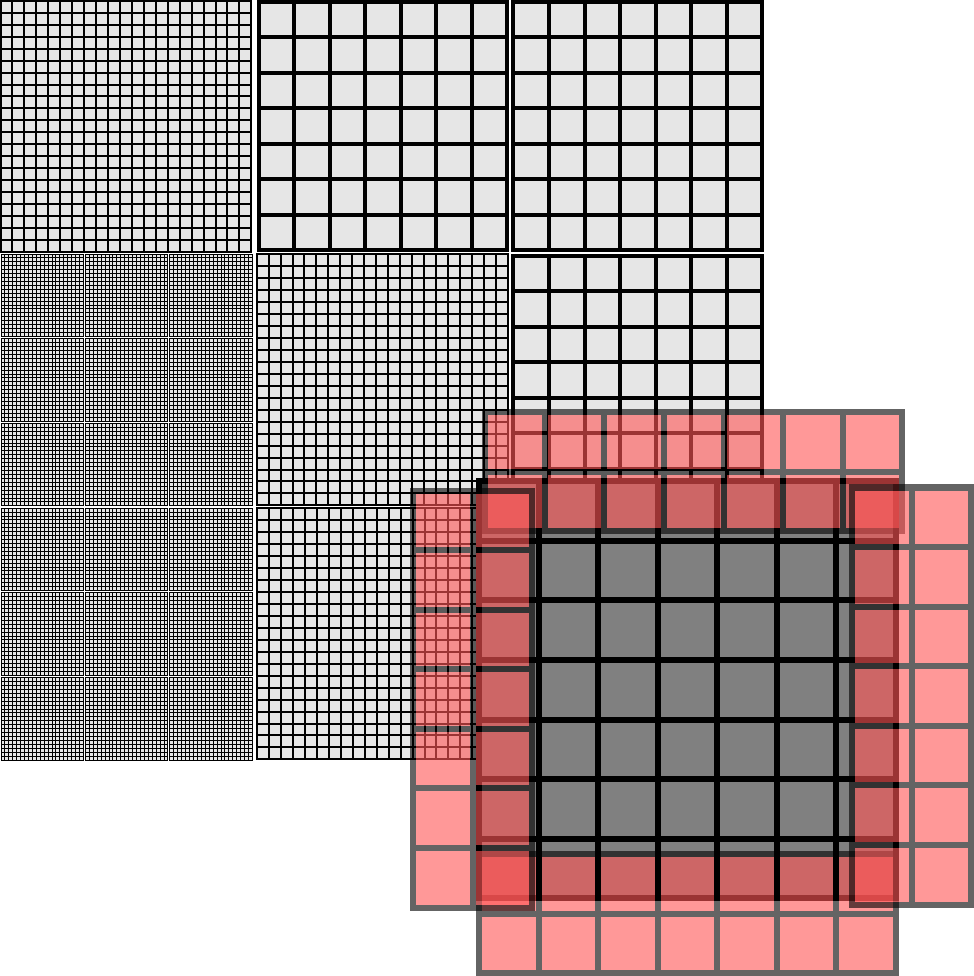
\includegraphics[width=0.5\textwidth]{42_finite-volumes/block-structured.pdf}
\end{center}

\begin{code}
project = peano4.Project( ["examples", "finitevolumes"], "." )
patch_size = 7
unknowns   = 5
patch = peano4.datamodel.Patch( (patch_size,patch_size,patch_size), unknowns, "Q" )
project.datamodel.add_cell(patch)
\end{code}

\noindent
In the above example, every volume within the $N \times N$ patches holds five
unknowns.
In general, I prefer the term volume here, as cell again is ambigous given that
we construct the \Peano\ host mesh from cells.


With one patch per cell, we could traverse the mesh and do something per cell.
This however is of limited value.
We have to couple the phenomena what is going on in neighbouring cells.
\Peano\  realises a strict element-wise traversal, i.e.~there's no way to access
the neighbour cell of a cell directly.
However, we can hijack the faces.


The idea here is that we embed a $2 \times N$ ($d=2$) or $2 \times N \times N$
($d=3$), respectively, patch into each face. 
Let this auxiliary patch overlap the adjacent cells.
Then, we effectively have a halo of one cell available within each cell:
We know the cell data. 
We also have access to the $2d$ faces where each hosts a degenerated patch.
One later of this patch is a copy of our own data, i.e.~does not give us
additional information.
The other layer of the auxiliary patch however holds data from the neighbour.
It gives us information from the neighbour patch.


In theory, we could only replicate those quantities that we really need. 
But it makes our live easier to just hold all five quantities in the auxiliary
face data structures, too:

\begin{code}
patch_overlap = peano4.datamodel.Patch( (2,patch_size,patch_size), unknowns, "Q" )
project.datamodel.add_face(patch_overlap)
\end{code}


Before we generate the code, we export some of the Python constants that we use
into C/C++, so we have it available there, too:

\begin{code}
project.constants.export( "PatchSize", patch_size )
project.constants.export( "NumberOfUnknownsPerCell", unknowns )
\end{code}


\section{Administration of the data structures}

Projecting the patches onto the face data structures and back is a mechnical
task.
Therefore, \Peano\  offers a toolbox to relieve you from the pain to 
recode it over and over again.
Using this toolbox, you add the projections to your algorithmic steps, and the
API then automatically injects these features (aspects) into your code:

\begin{code}
perform_time_step      = peano4.solversteps.Step( "TimeStep" )
perform_time_step.use_cell(patch)
perform_time_step.use_face(patch_overlap)
...
perform_time_step.add_action_set( 
  peano4.toolbox.blockstructured.ReconstructPatchAndApplyFunctor(patch,patch_overlap,...)
) 
perform_time_step.add_action_set( 
  peano4.toolbox.blockstructured.ProjectPatchOntoFaces(patch,patch_overlap) 
)
\end{code}



\begin{center}
  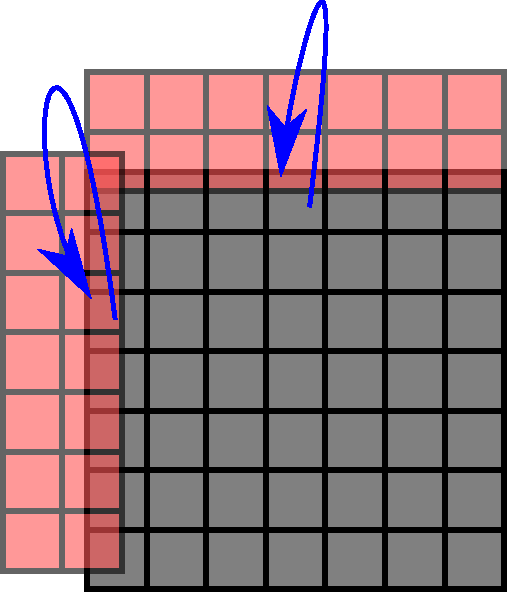
\includegraphics[width=0.25\textwidth]{42_finite-volumes/ProjectPatchOntoFaces.pdf}
\end{center}


\noindent
The image above illustrates what \texttt{ProjectPatchOntoFaces} does:
It knows the dimensions of both the patches and the face auxiliary data
structures and thus can ensure that the right data is copied from the cell into
the $2^d$ faces when we leave a cell throughout the grid traversal.



The action set \texttt{ReconstructPatchAndApplyFunctor} works slighlty different
yet can be read, from a patch projection point of view, as transpose of
\texttt{ProjectPatchOntoFaces}:
It creates a auxiliary variable \texttt{reconstructedX} with X being the name
you gave the Unknowns of the patch.
This auxiliary variable has the dimensions 
$N+2 \times N+2 \times N+2$\footnote{All tools work with overlaps greater than
2. But to keep the text simple, I stick to 2.}.
It then copies over the patch data into this auxiliary patch and uses the faces
to supplement it with halo data around it.
So that it, you get the original patch data plus the cells around it in one big
patch.


\section{A manually implemented FV scheme}

As the name suggests, the reconstruction step is typically combined with the
invocation of some computation on the patch.
We give a simple example of a Finite Volume solver for the Euler equations here.


Once a patch is reconstructed, we have a huge double array (AoS) of the
reconstructed patch, i.e.~the patch plus its surrounding halo, available.
It holds a copy of the actual patch data.
This patch data is still available as well, so we can use the reconstructed
array as a preimage and write any outcome into the patch data structure.


We begin with defining a simple functor implementing this PDE plus a very simple
Rusanov flux:
\begin{code}
auto eigenvalues = [](double Q[5], const tarch::la::Vector<Dimensions,double>& x, 
  int normal, double lambda[5]
) -> void {
  constexpr double gamma = 1.4;
  const double irho = 1./Q[0];
  #if Dimensions==3
    const double p = (gamma-1) * (Q[4] - 0.5*irho*Q[1]*Q[1]+Q[2]*Q[2]+Q[3]*Q[3]);
  #else
    const double p = (gamma-1) * (Q[4] - 0.5*irho*Q[1]*Q[1]+Q[2]*Q[2]);
  #endif

  const double u_n = Q[normal + 1] * irho;
  assertion10( gamma * p * irho>=0.0, gamma, p, irho, x, normal, Q[0], Q[1], Q[2], Q[3], Q[4] );
  const double c   = std::sqrt(gamma * p * irho);

  lambda[0]  = u_n;
  lambda[1]  = u_n;
  lambda[2]  = u_n;
  lambda[3]  = u_n + c;
  lambda[4]  = u_n - c;
    
  assertion4( lambda[0]==lambda[0], u_n, c, x, normal );
  assertion4( lambda[1]==lambda[1], u_n, c, x, normal );
  assertion4( lambda[2]==lambda[2], u_n, c, x, normal );
  assertion4( lambda[3]==lambda[3], u_n, c, x, normal );
  assertion4( lambda[4]==lambda[4], u_n, c, x, normal );
};
  
auto flux = [](
  double Q[5], const tarch::la::Vector<Dimensions,double>& x, int normal, double F[5]
) -> void {
  assertion5( Q[0]==Q[0], Q[0], Q[1], Q[2], Q[3], Q[4] );    
  assertion5( Q[1]==Q[1], Q[0], Q[1], Q[2], Q[3], Q[4] );    
  assertion5( Q[2]==Q[2], Q[0], Q[1], Q[2], Q[3], Q[4] );    
  assertion5( Q[3]==Q[3], Q[0], Q[1], Q[2], Q[3], Q[4] );    
  assertion5( Q[4]==Q[4], Q[0], Q[1], Q[2], Q[3], Q[4] );    
    
  assertion5( Q[0]>1e-12, Q[0], Q[1], Q[2], Q[3], Q[4] );
  constexpr double gamma = 1.4;
  const double irho = 1./Q[0];
  #if Dimensions==3
    const double p = (gamma-1) * (Q[4] - 0.5*irho*Q[1]*Q[1]+Q[2]*Q[2]+Q[3]*Q[3]);
  #else
    const double p = (gamma-1) * (Q[4] - 0.5*irho*Q[1]*Q[1]+Q[2]*Q[2]);
  #endif

  switch (normal) {
    case 0:
      {
        F[0] = Q[1];
        F[1] = irho*Q[1]*Q[1] + p;
        F[2] = irho*Q[2]*Q[1];
        F[3] = (Dimensions==3) ? irho*Q[3]*Q[1] : 0.0;
        F[4] = irho*(Q[4]+p)*Q[1];
      }
      break;
    case 1:
      {
        F[0] = Q[2];
        F[1] = irho*Q[1]*Q[2];
        F[2] = irho*Q[2]*Q[2] + p;
        F[3] = (Dimensions==3) ? irho*Q[3]*Q[2] : 0.0;
        F[4] = irho*(Q[4]+p)*Q[2];
      }
      break;
    case 2:
      {
        F[0] = Q[3];
        F[1] = irho*Q[1]*Q[3];
        F[2] = irho*Q[2]*Q[3];
        F[3] = (Dimensions==3) ? irho*Q[3]*Q[3] + p : 0.0;
        F[4] = irho*(Q[4]+p)*Q[3];
      }
      break;
  }

  assertion( F[0]==F[0] );
  assertion( F[1]==F[1] );
  assertion( F[2]==F[2] );
  assertion( F[3]==F[3] );
  assertion( F[4]==F[4] );
};

auto splitRiemann1d = [&flux, &eigenvalues](
  double QL[5], double QR[5], const tarch::la::Vector<Dimensions,double>& x,
  double dx, double dt, int normal, double F[5]
) -> void { double averageQ[5]; 
  for (int unknown=0; unknown<5; unknown++) {
    averageQ[unknown] = 0.5 * (QL[unknown] + QR[unknown]);    
  }
    
  double averageF[5];
  double lambdas[5];
  flux(averageQ,x,normal,averageF);
  
  double lambdaMax = 0.0;
  eigenvalues(averageQ,x,normal,lambdas);
  for (int unknown=0; unknown<5; unknown++) {
    lambdaMax = std::max(lambdaMax,lambdas[unknown]);
  }
  
  for (int unknown=0; unknown<5; unknown++) {
    F[unknown] = averageF[unknown] - 0.5 * lambdaMax * (QR[unknown] - QL[unknown]);
  }
};  
\end{code}

\noindent
Let all of this be one string assigned to a variable \texttt{functor}.


So this string now contains all the helpers we need to realise a Finite Volume
scheme, but it does not yet implement the scheme itself.
This is the final loop that's missing, and we can directly attach it to the
functor and then pass over to the reconstruction aspect:

\begin{code}
  constexpr int PatchSize = 13;
  constexpr int HaloSize  = 1;    
  double dt = 0.0001;
  assertion( dx>=tarch::la::NUMERICAL_ZERO_DIFFERENCE );
  dfor(cell,PatchSize) { // DOFS_PER_AXIS
    tarch::la::Vector<Dimensions,double> voxelCentre = centre 
      - static_cast<double>((PatchSize/2+HaloSize)) * tarch::la::Vector<Dimensions,double>(dx) 
      + tarch::la::multiplyComponents(cell.convertScalar<double>(), tarch::la::Vector<Dimensions,double>(dx));
    
    tarch::la::Vector<Dimensions,int> currentVoxel = cell + tarch::la::Vector<Dimensions,int>(HaloSize); // OVERLAP / Halo layer size
    int currentVoxelSerialised = peano4::utils::dLinearised(currentVoxel,PatchSize + 2*HaloSize);
    
    double accumulatedNumericalFlux[] = { 0.0, 0.0, 0.0, 0.0, 0.0 };
  ...
  }
\end{code}


\section{Plot results}

For the plotting of patch-based AMR, \Peano\ provides predefined action sets,
too.
They dump the output into Peano's patch format.
Chapter \ref{capter:blockstructured-output-format} describes this format. 
If you build your code with VTK support, \Peano\ offers a conversion script into
VTK.



To use the predefined file dump feature, add an instance of
\texttt{PlotPatchesInPeanoBlockFormat} to the step of your choice. 
It then looks similar to
\begin{code}
print_solution = peano4.solversteps.Step( "PlotSolution" )
print_solution.use_cell(patch)
print_solution.use_face(patch_overlap)
print_solution.remove_all_actions()
plotter = peano4.toolbox.blockstructured.PlotPatchesInPeanoBlockFormat("solution",patch,"Q")
print_solution.add_action_set( plotter )
project.solversteps.add_step(print_solution)
\end{code}





